\chapter{Battery Monitor for AAUSHIP}
\label{ch:bm}

\head{This appendix is a minor chapter describing a hardware
	component, the battery monitor, for AAUSHIP which was also devised
	under the project period. This is not directly a goal according to
	the project thesis, hence this is included in the appendix as
	reference.}

Since the AAUSHIP is equipped with multiple LiPo cells, it is of high concern to have a means of checking the state of these battery cells.
Therefore a battery monitor have been created, that can be hooked onto the
\ac{LLI} via the I$^2$C bus. This will enable the \ac{HLI} to report
the voltages on the cells. This was implemented with \ac{ROS} by
utilizing the graphical interface for \ac{ROS} called rqt. In this Qt
based environment it is possible to make plugins as easy as it is to
create \ac{ROS} nodes. A screenshot of the plugin in action is seen
on figure~\vref{fig:bm-rqt}.

The battery monitor is made of two \ac{ADC} chips, namely the MCP3428,
each with four channels and 16-bit resolution. But not all this
resolution is of real use as such, because it is implemented with a
resistor voltage divider from each cell in series, which basically
means that only the top end of the value range is used. 

It is designed to measure maximum 4.2 V per cell to the minimum
allowed voltage of about 3.6 V per cell. It can of course measure
smaller values but the critical value is around 3.6 V. The four cells are connected in series, each with a resistor divider with
reference to the negative lead. The division ratio is determined by
the maximum voltage present at the cells (which are in series with the
lower ones), such that the cell voltages are at the two volt that
each \ac{ADC} can handle. This gives the following ratios for the
cells:
\begin{align}
	\#1 = 0.12, \quad \#2 = 0.16, \quad \#3 = 0.24, \quad \#4 = 0.48
\end{align}

This means that the voltage on high cell \ac{ADC} is ranging from
about 1.728 V to 2.0 V. In turn meaning that the reading will only use
the top 15 \% of the capabilities of the \ac{ADC}. This results in a
range for the high side \ac{ADC} of about 288 when using the exact
numbers, which equates to about 8 mV per \ac{LSB}. The lower ranges
are more accurate.

High resistance dividers is used since these are always connected to
the battery, and the resistance is adjusted such that the discharge
current is very low, in comparison to the self discharge of the
battery. The highest discharge rate for the cells are 138 µA, which
corresponds to a fully charged pack to discharge over three years.
Note if needed to store the batteries for a significant amount of
time they should be disconnected completely.

On the following pages are the printed circuit board and schematic attached.

\begin{figure}[H]
	\centering
	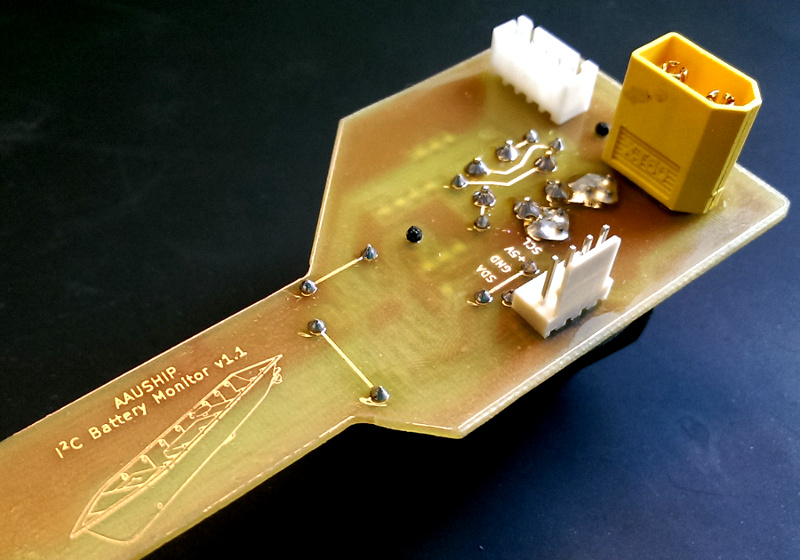
\includegraphics[width=0.8\textwidth]{fig/bm-macro}
	\caption{Macro photo of the finished battery monitor.}
	\label{fig:bm-macro}
\end{figure}

\begin{figure}[H]
	\centering
	\includegraphics[width=\textwidth]{fig/bm-rqt}
	\caption{Screen shot of the battery monitor plugin in rqt.}
	\label{fig:bm-rqt}
\end{figure}

\includepdf{pdf/bm-pcb}
\includepdf[angle=90]{pdf/bm-sch}
